\documentclass[12pt]{article}
\usepackage{fullpage,enumitem,amsmath,amssymb,graphicx}

\begin{document}

\begin{center}
{\Large CS221 Fall 2018 Homework [car]}

\begin{tabular}{rl}
SUNet ID: & prabhjot \\
Name: & Prabhjot Singh Rai
\end{tabular}
\end{center}

By turning in this assignment, I agree by the Stanford honor code and declare
that all of this is my own work.

\section*{Problem 1}

\begin{enumerate}[label=(\alph*)]
  \item 
  \textbf{Step 1: Remove variables that are not ancestors} \\
  \textbf{Step 2: Converting to factor graph} \\
  Step 1 and step 2 are shown in diagram below:
  \begin{center}
  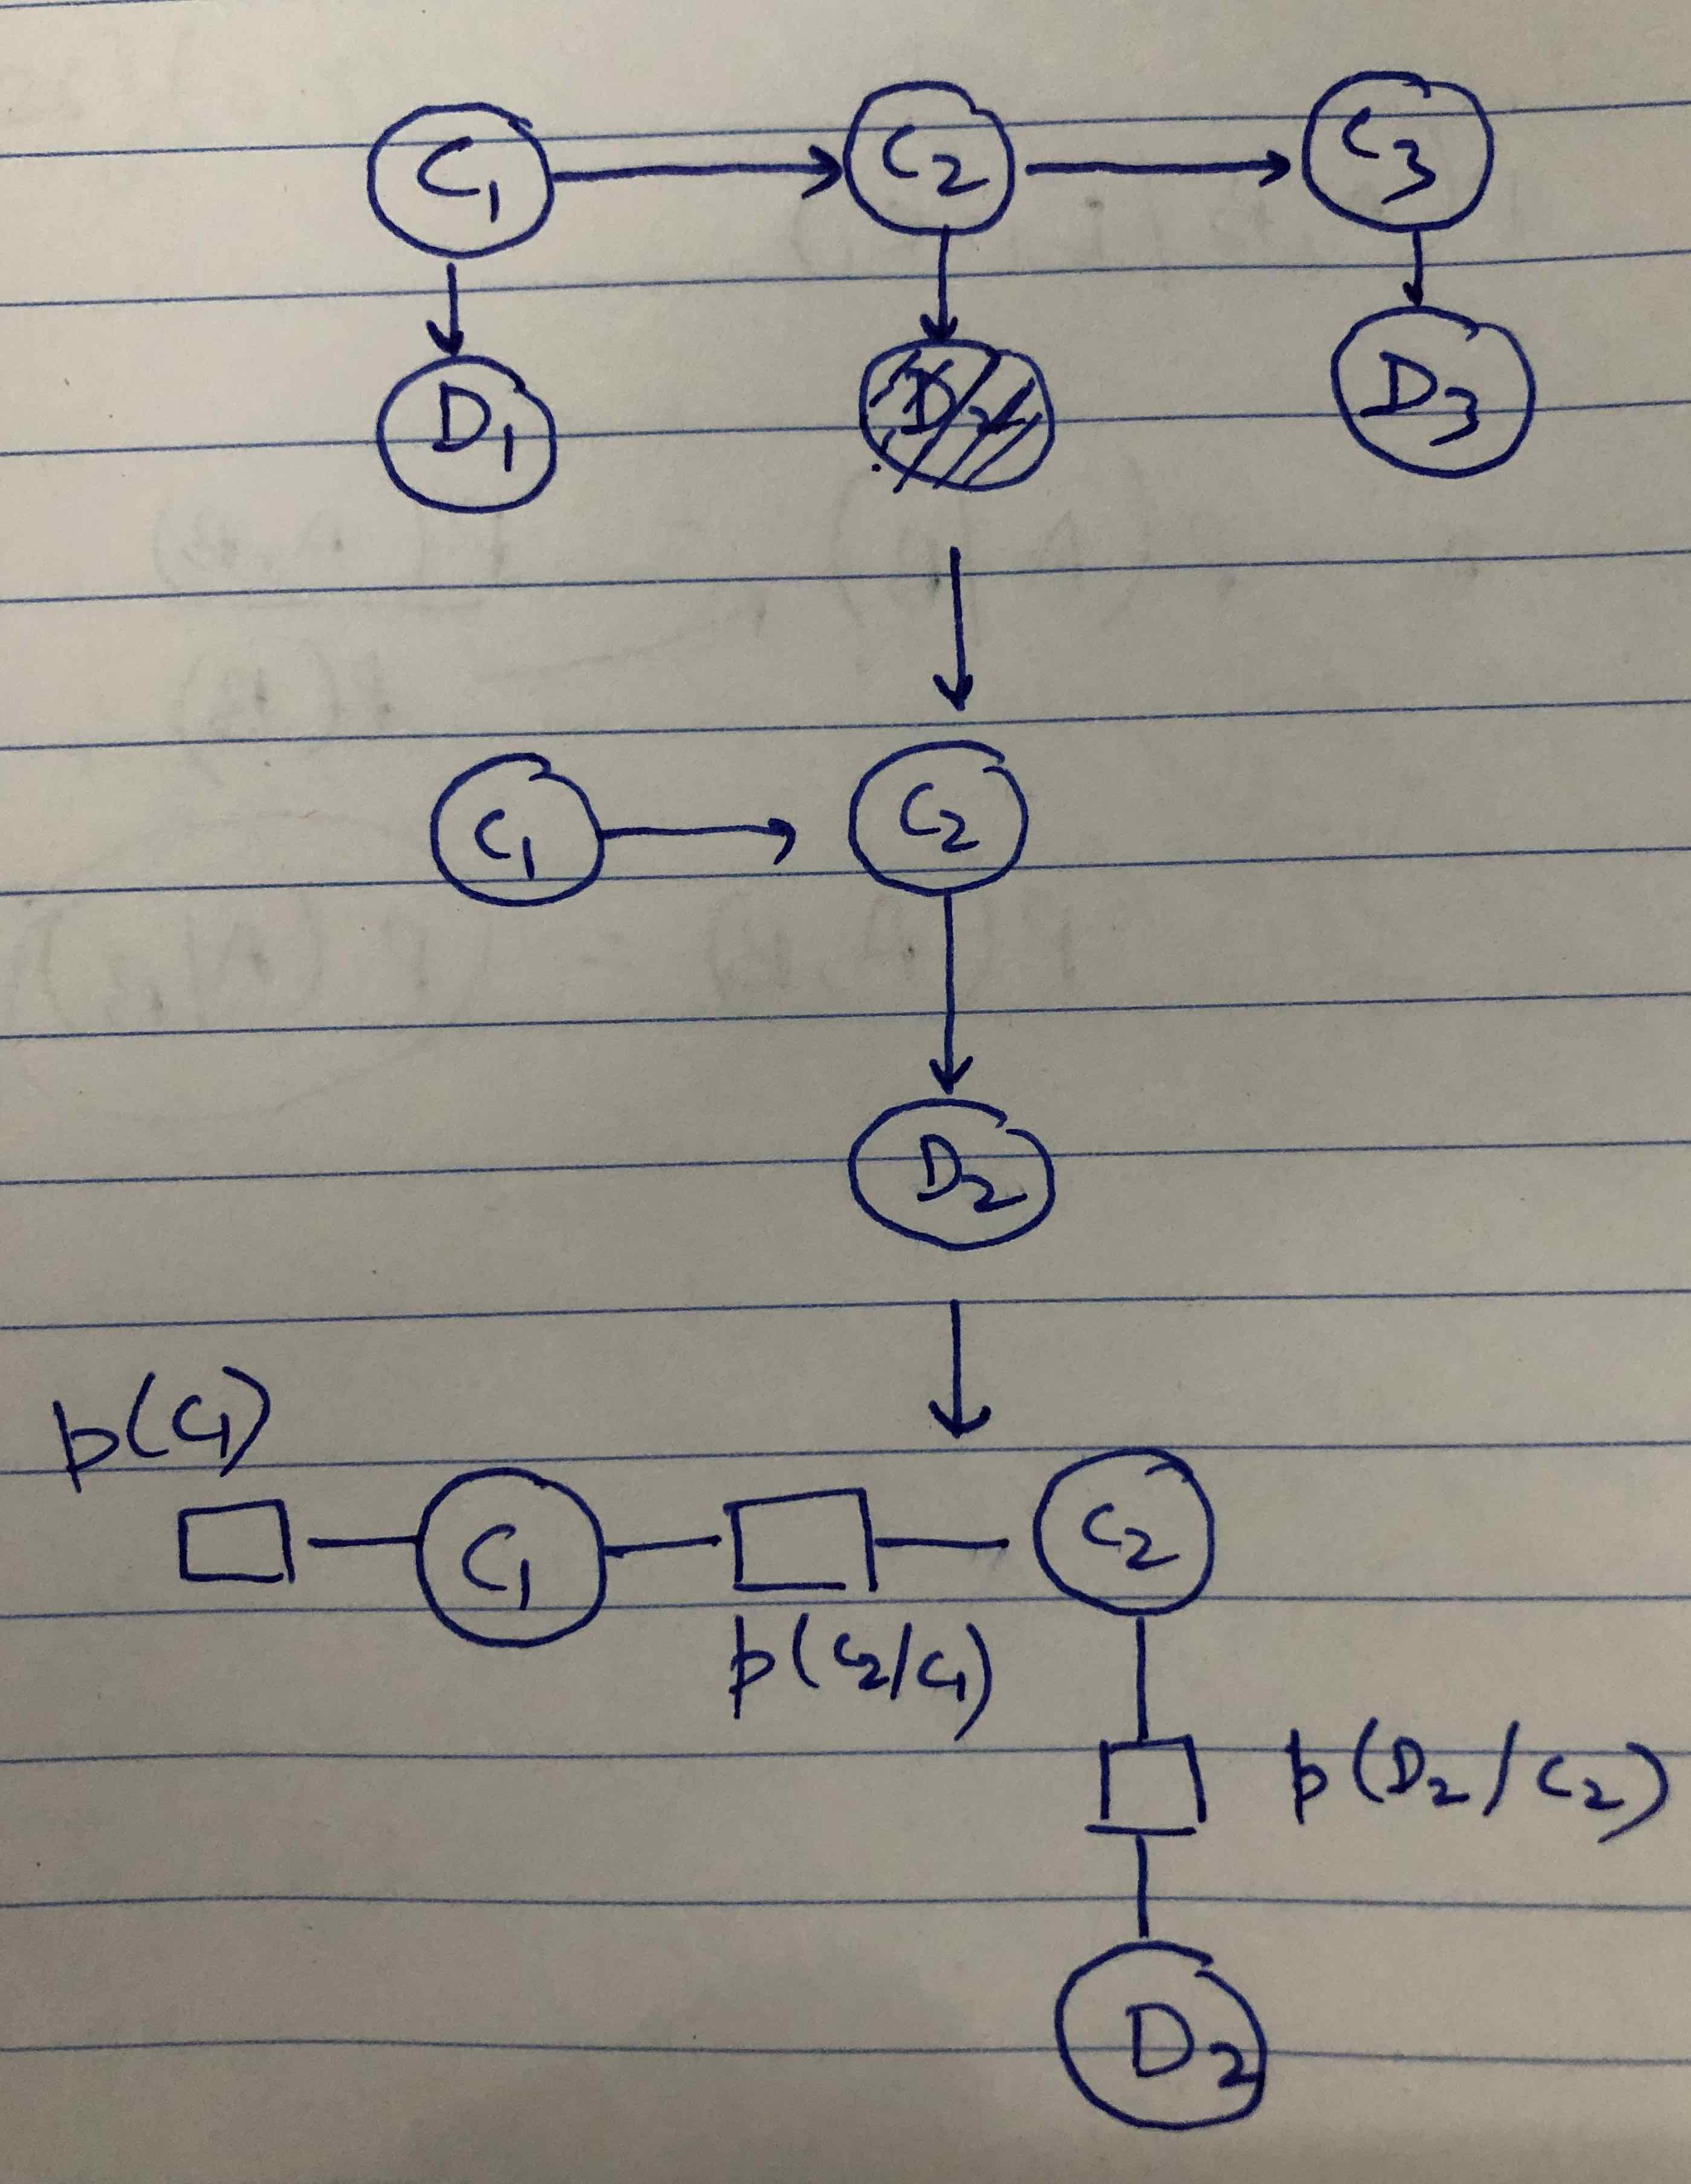
\includegraphics[scale=0.1]{IMG_2276}
  \end{center}
  \textbf{Step3: Conditioning on $D_2 = 0$} \\
  \begin{center}
  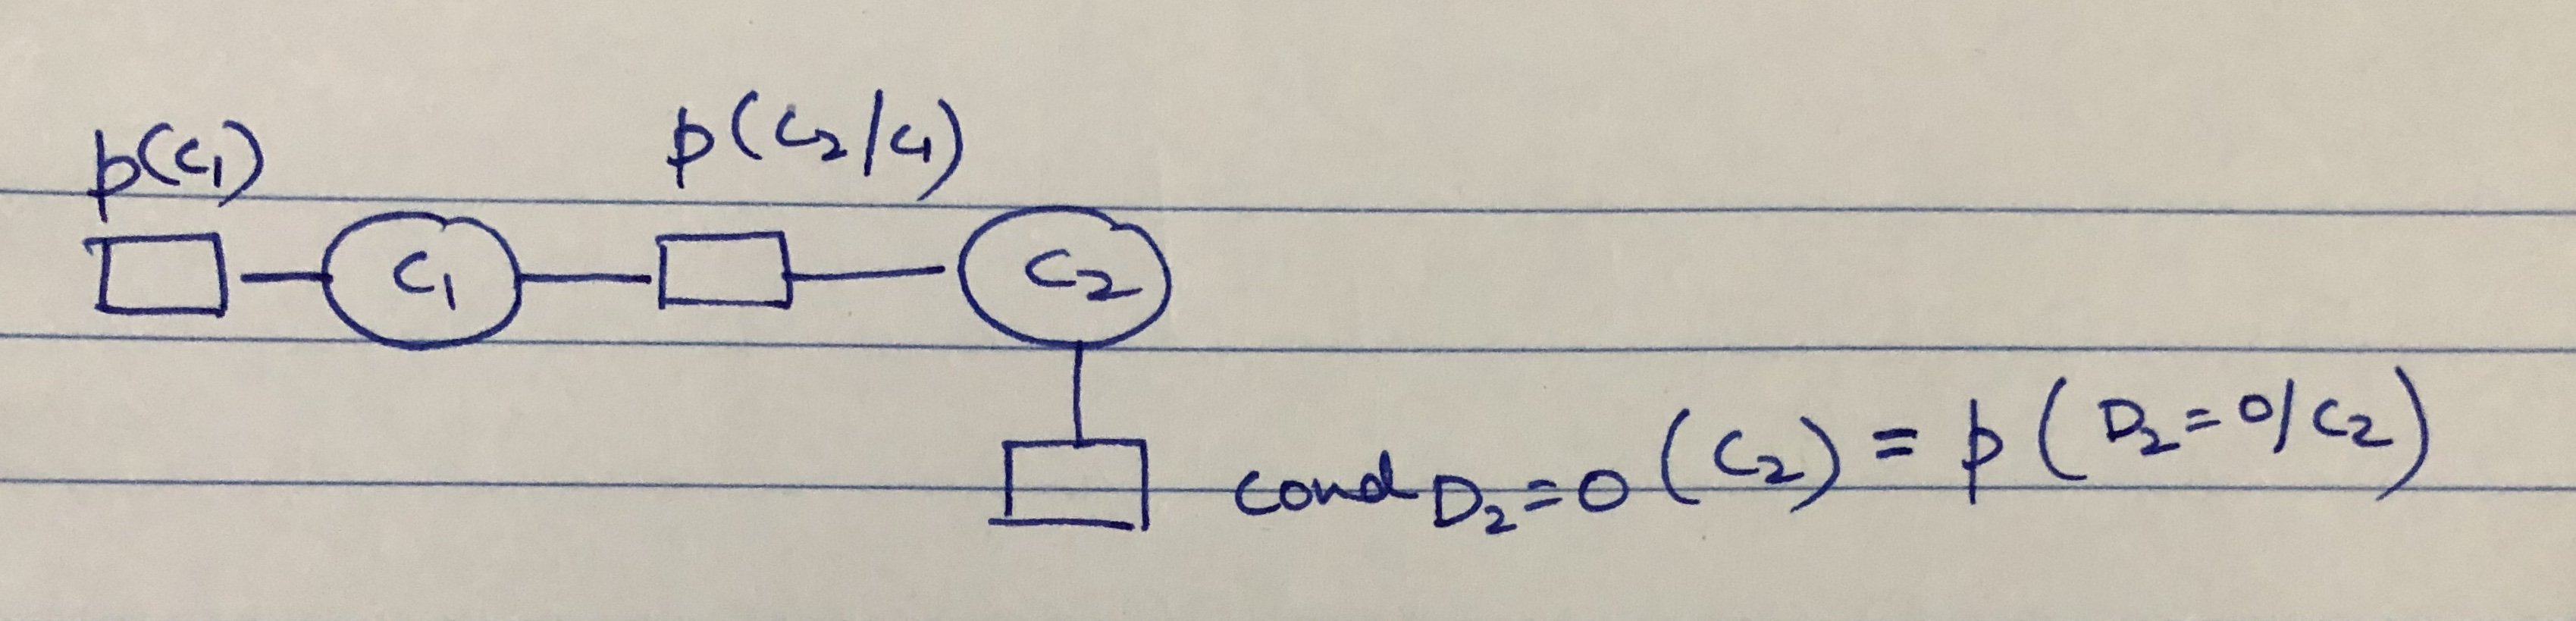
\includegraphics[scale=0.1]{IMG_2278.jpg}
  \end{center}
  Condition variable $D_2$ on value $D_2 = 0$, replacing it with a factor cond$_{D_2 = 0}(C_2)$, we get
  \begin{center}
  \begin{tabular}{ll}
  cond$_{D_2 = 0}(C_2)$ & $C_2$  \\
  $1-\eta$            & 0       \\
  $\eta$               & 1       \\
  \end{tabular} \newline \\
  \end{center}
  \textbf{Step4: Eliminate $C_1$} \\
  \begin{center}
  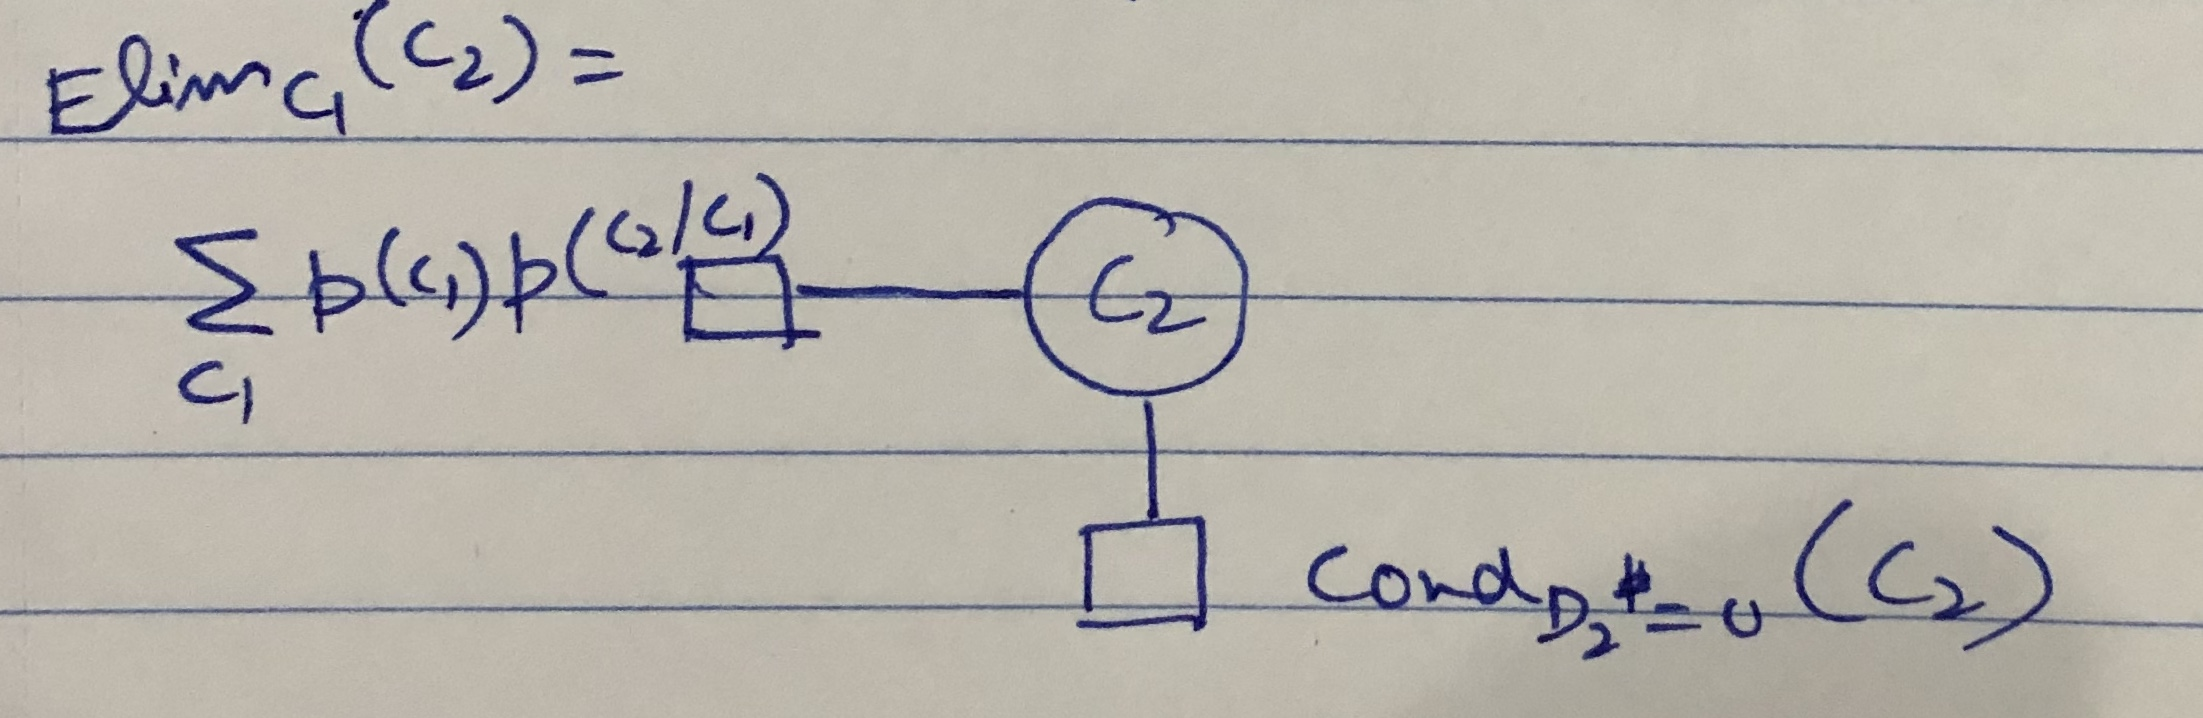
\includegraphics[scale=0.1]{IMG_2277.jpg}
  \end{center}
  \begin{align*}
	elim_{C_1}(C_2) &= \sum_{C_1} p(C_1) p(C_2/C_1) \\
	&= 0.5 \sum_{C_1} p(C_2/C_1)
  \end{align*}
  This is given from the below table:
  \begin{center}
  \begin{tabular}{ll}
  elim$_{C_1}(C_2)$ & $C_2$  \\
  $0.5(1-\epsilon + \epsilon) = 0.5$            & 0       \\
  $0.5(\epsilon + 1-\epsilon) = 0.5$               & 1       \\
  \end{tabular} \newline \\
  \end{center}
  Therefore, now that we know elim$_{C_1}(C_2)$ and cond$_{D_2 = 0} (C_2)$,
  \begin{align*}
  p(C_2/ D_2 = 0) &= \text{elim}_{C_1}(C_2) * \text{cond}_{D_2 = 0} (C_2)
  \end{align*}
  \begin{center}
  \begin{tabular}{ll}
  $p(C_2/ D_2 = 0)$ & $C_2$  \\
  $0.5 (1-\eta)$            & 0       \\
  $0.5 \eta$               & 1       \\
  \end{tabular} \newline \\
  \end{center}
  Hence, the given query,
  \begin{align*}
  p(C_2 = 1/ D_2 = 0) &= \frac{0.5 \eta}{0.5 \eta + 0.5 (1-\eta)} \\
  &= \eta
  \end{align*}
  \item 
  \textbf{Step1: Remove variables that are not ancestors} \\
  \textbf{Step2: Converting to factor graph} \\
  Step 1 and step 2 are illustrated below:
  \begin{center}
  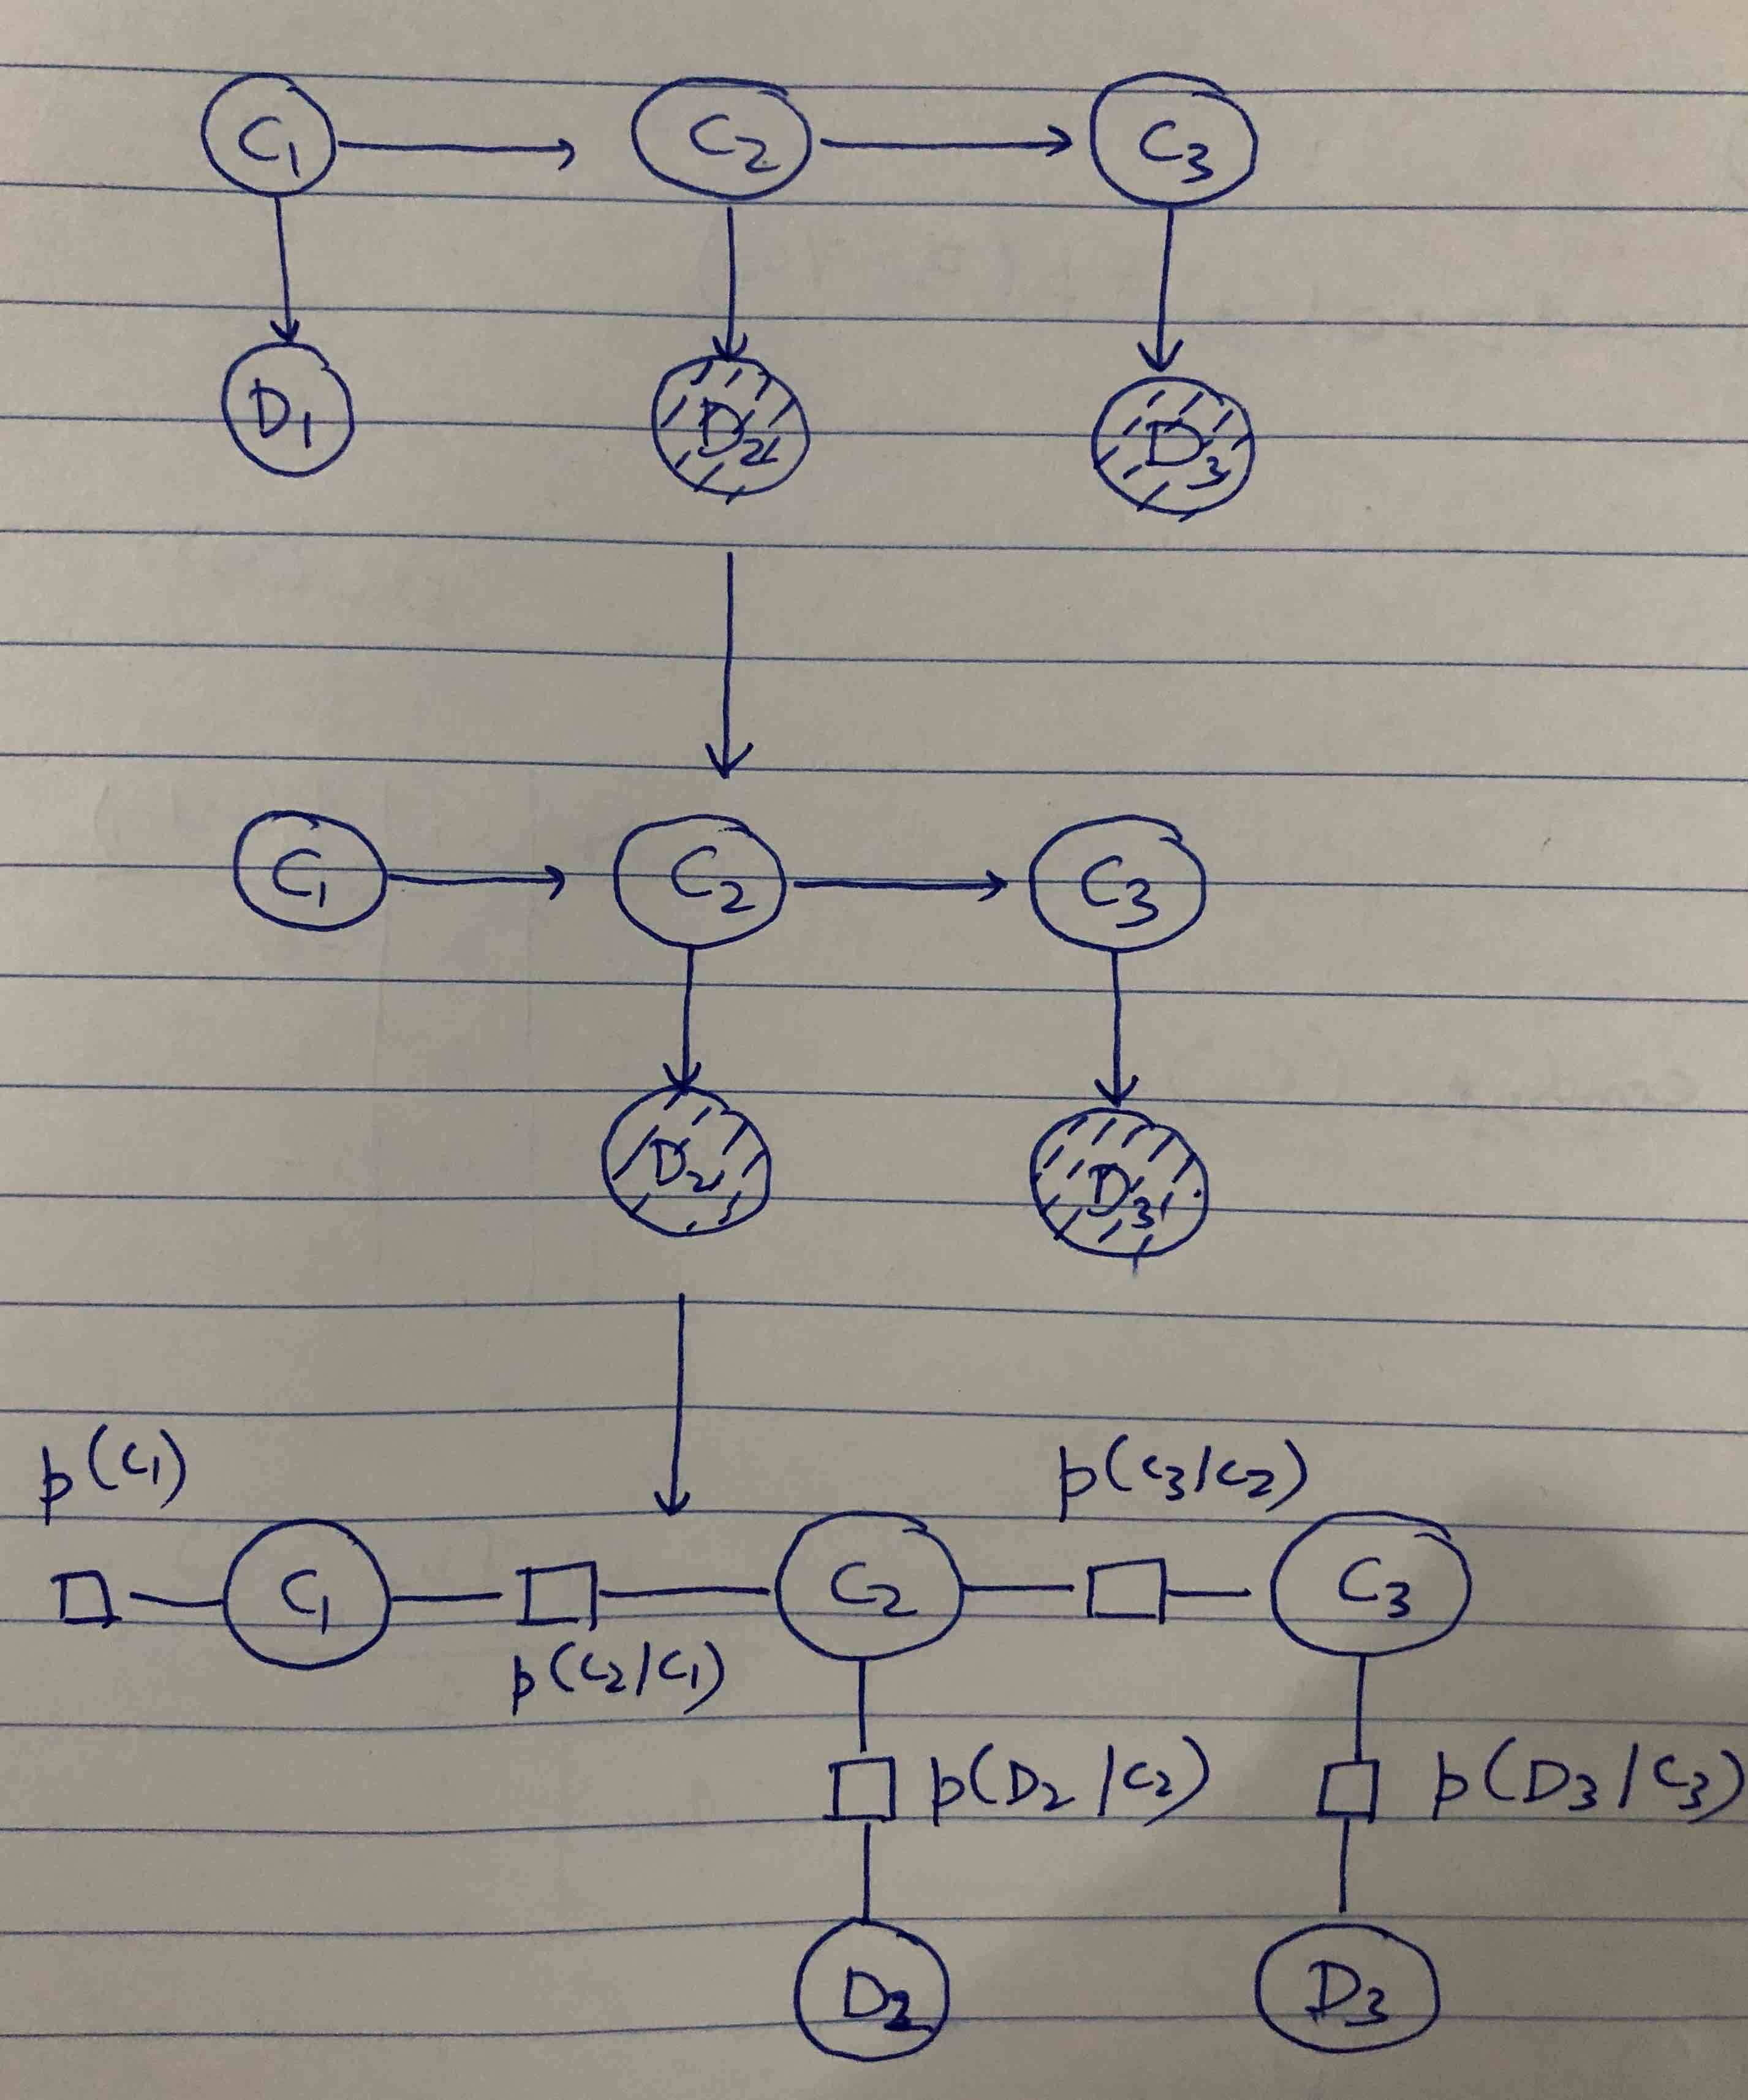
\includegraphics[scale=0.1]{IMG_2279.jpg}
  \end{center}
  \textbf{Step3: Conditioning on $D_3 = 1$} \\
  \begin{center}
  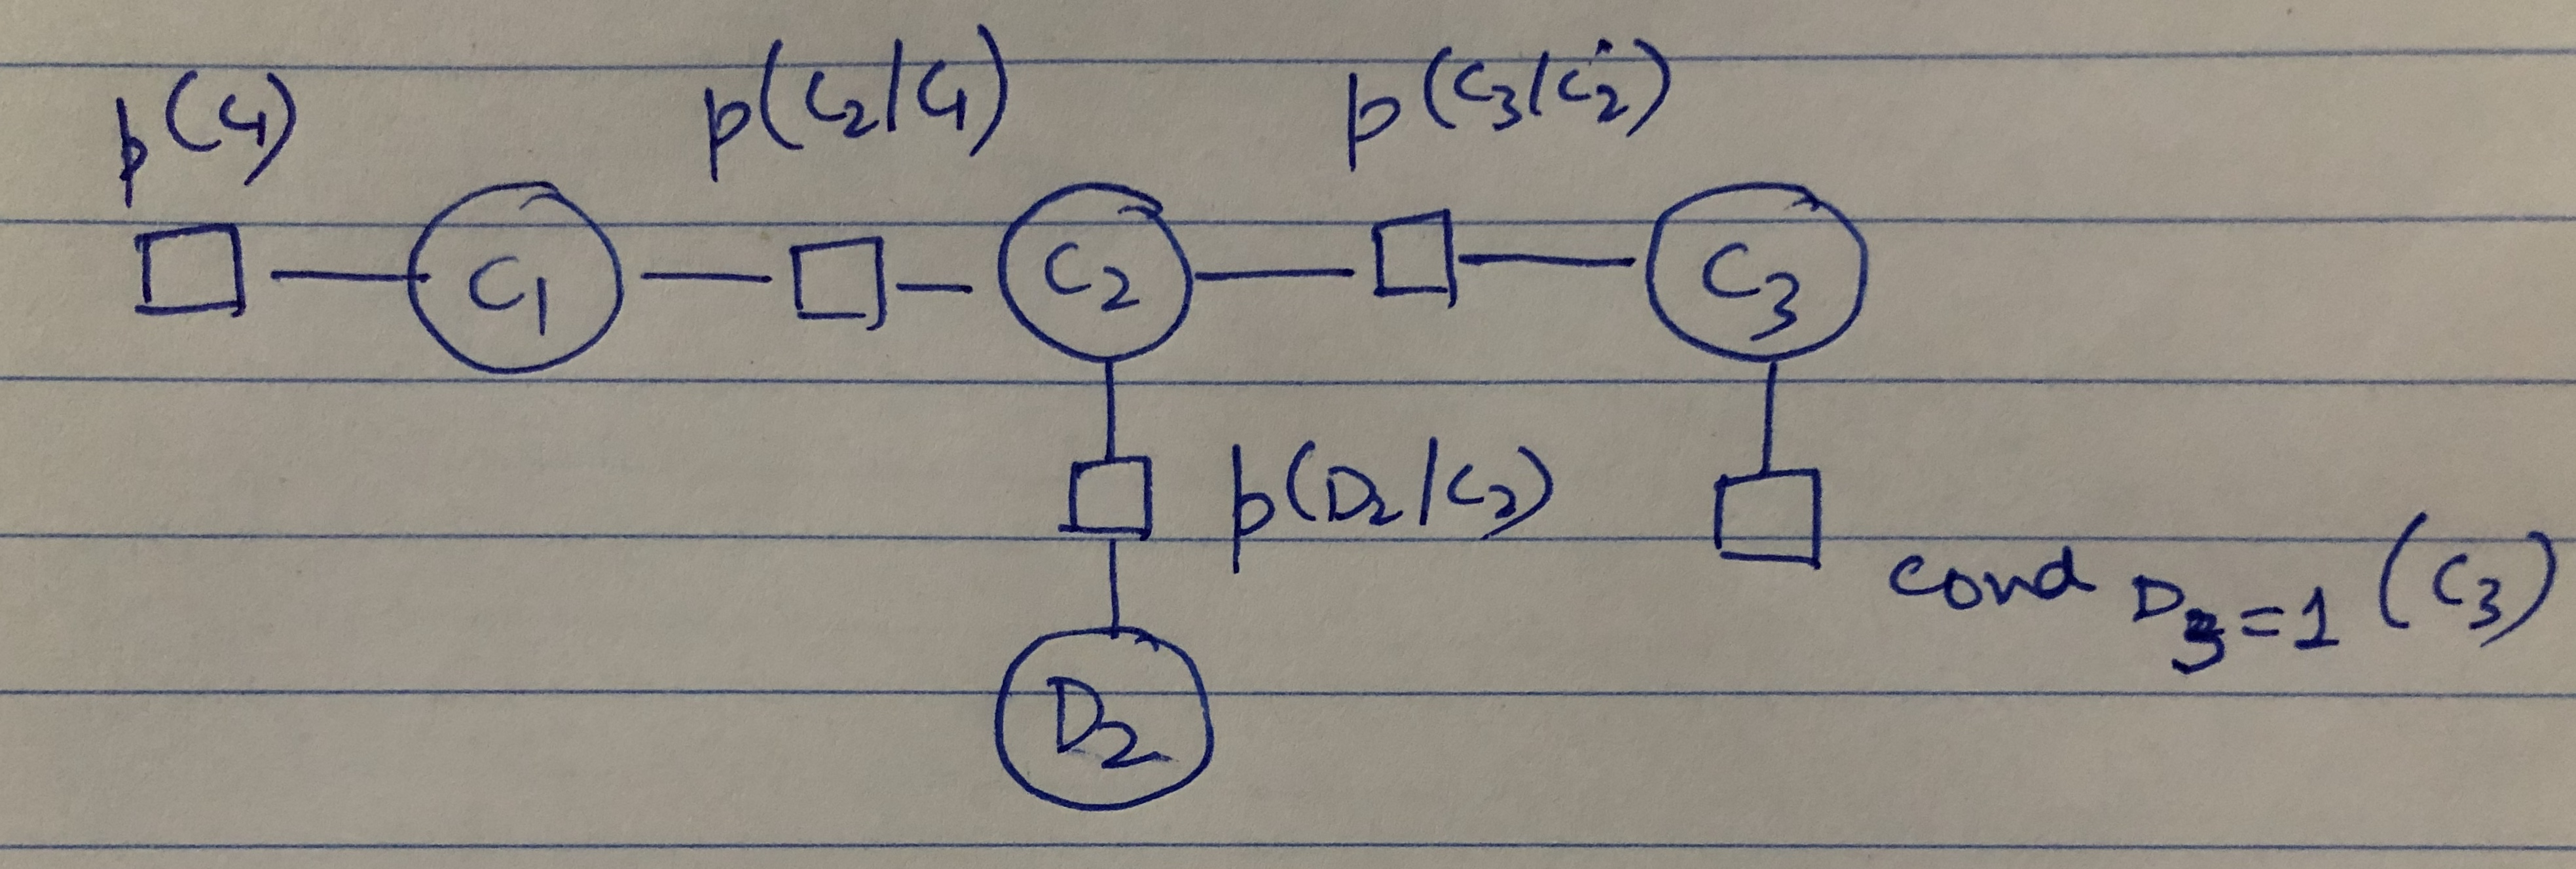
\includegraphics[scale=0.1]{IMG_2280.jpg}
  \end{center}
  Conditioning on variable $D_3$, and replacing it with a factor cond$_{D_3 = 1}(C_3)$, we get
  \begin{center}
  \begin{tabular}{ll}
  cond$_{D_3 = 1}(C_3)$ & $C_3$  \\
  $\eta$            & 0       \\
  $1-\eta$               & 1       \\
  \end{tabular} \newline \\
  \end{center}
  \textbf{Step4: Eliminating $C_3$}
  \begin{center}
  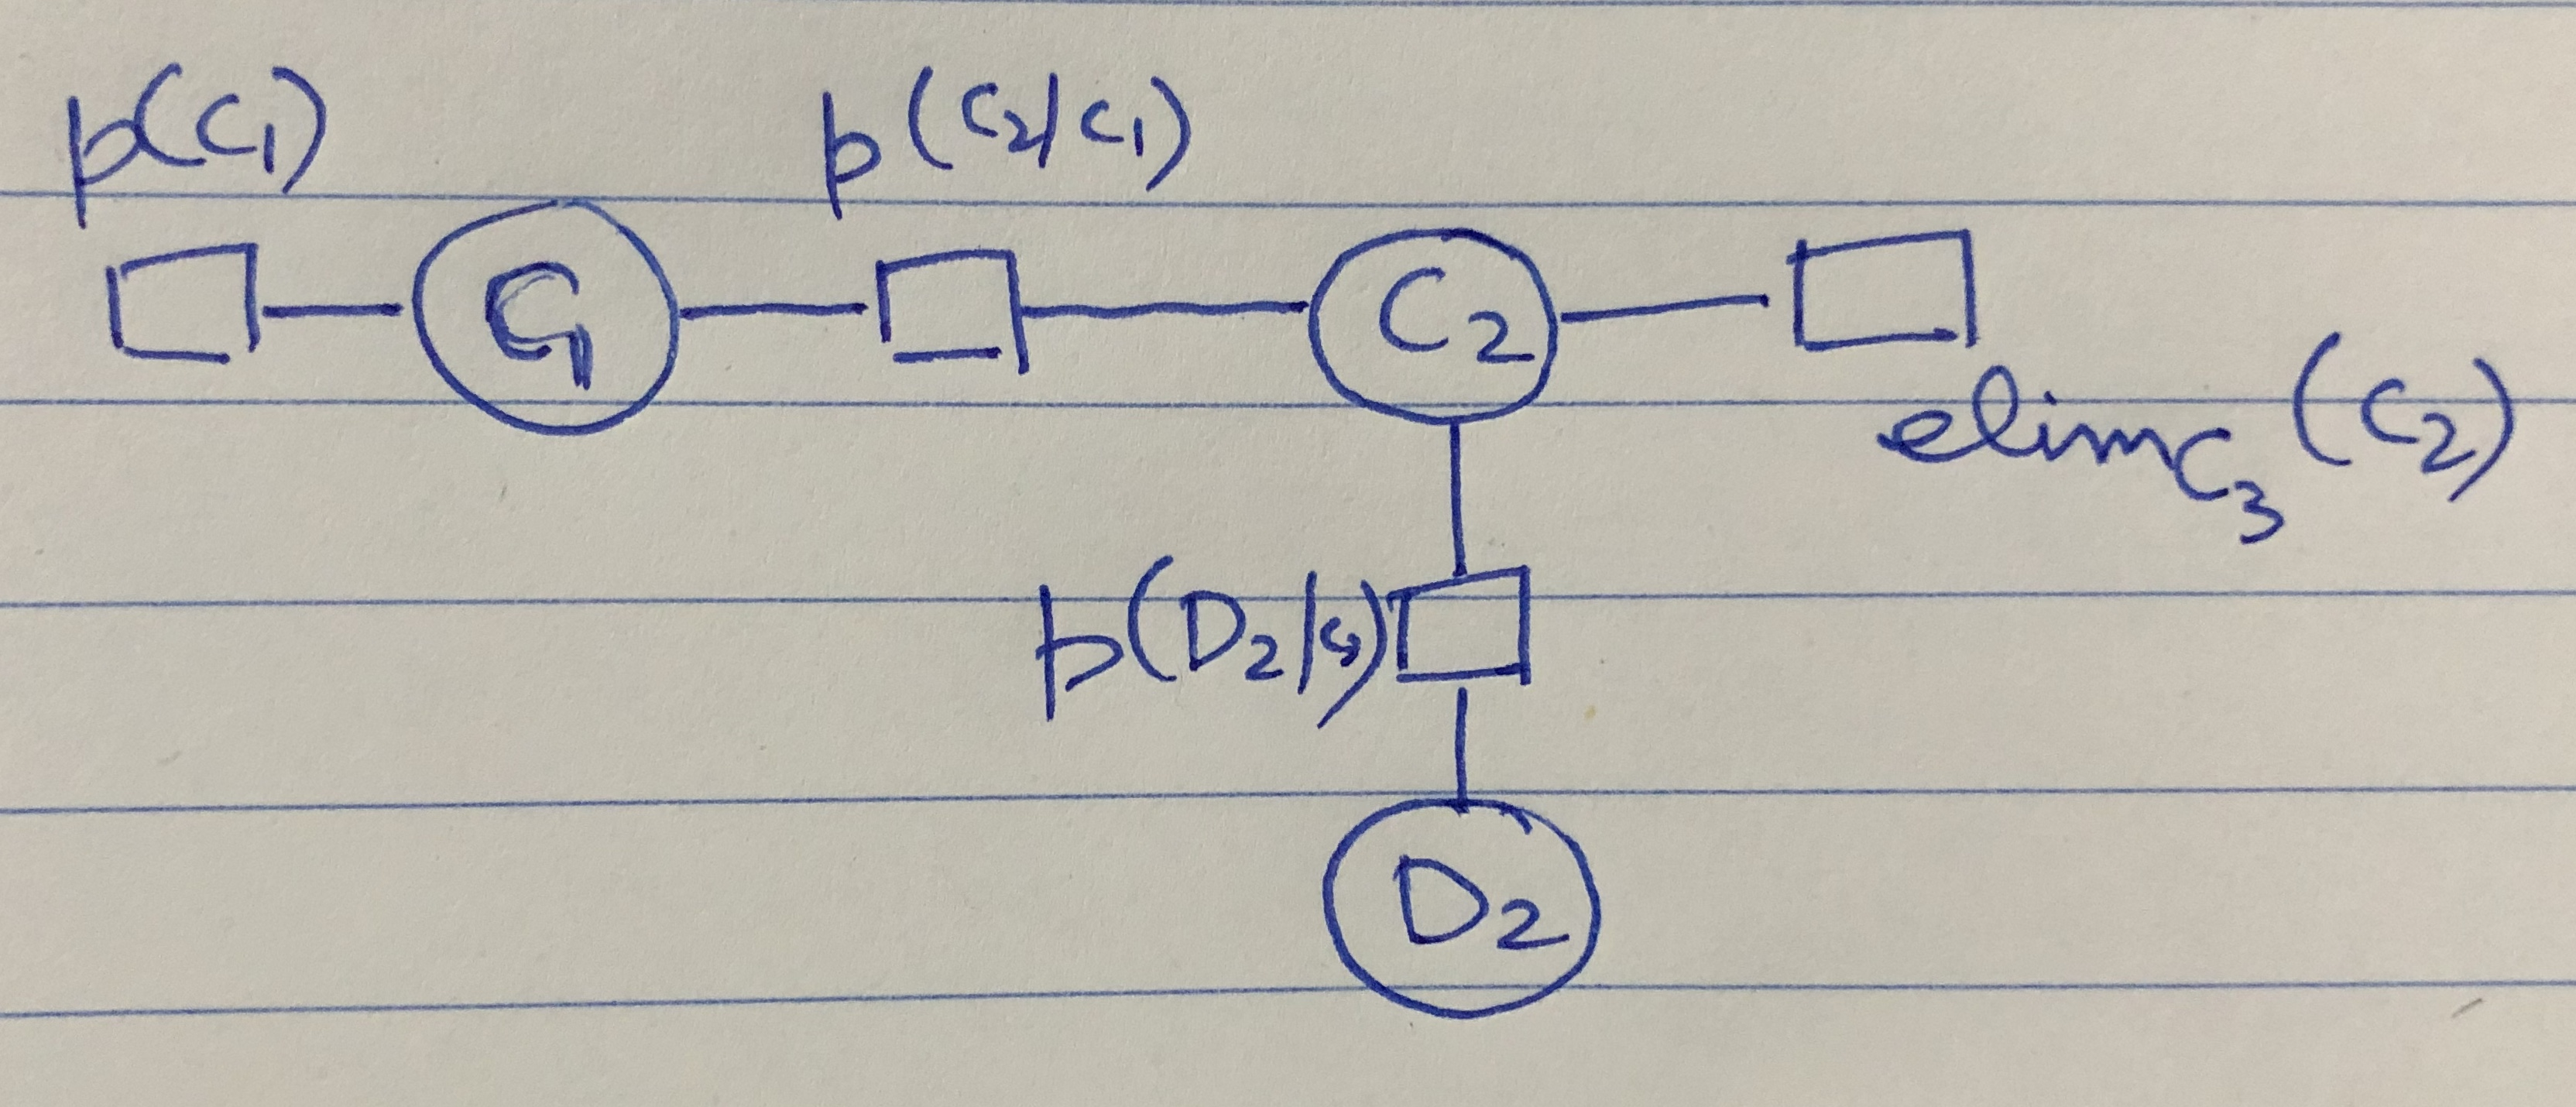
\includegraphics[scale=0.1]{IMG_2281.jpg}
  \end{center}
  Defining function elim$_{C_3}(C_2)$ in order to eliminate node $C_3$ as
  \begin{align*}
  \text{elim}_{C_3}(C_2) = \sum_{C_3} \text{cond}_{D_3 = 1}(C_3) p(C_3/C_2)
  \end{align*}
  The probability distribution $p(C_3/C_2)$ is given by:
  \begin{center}
  \begin{tabular}{lll}
  C2 & C3 & p(C3/C2)    \\
  0  & 0  & $1 - \epsilon$  \\
  0  & 1  & $\epsilon$      \\
  1  & 0  & $\epsilon$      \\
  1  & 1  & $1 - \epsilon$
  \end{tabular}
  \end{center}
  The probability distribution cond$_{D_3 = 1}(C_3)$ is defined in Step 3.
  
  Combining both and substituting in equation 1, and doing summation over values of $C_3$, we will have probability distribution of elim$_{C_3}(C_2)$ is given by:
  \begin{center}
  \begin{tabular}{ll}
  $C_2$ & elim$_{C_3}(C_2)$                               \\
  0  & $(1 - \epsilon) \eta + \epsilon (1- \eta)$   \\
  1  & $\epsilon \eta + (1- \eta) (1 - \epsilon)$ 
  \end{tabular}
  \end{center}
  
  \textbf{Step5: Conditioning on $D_2 = 0$} \\
  \begin{center}
  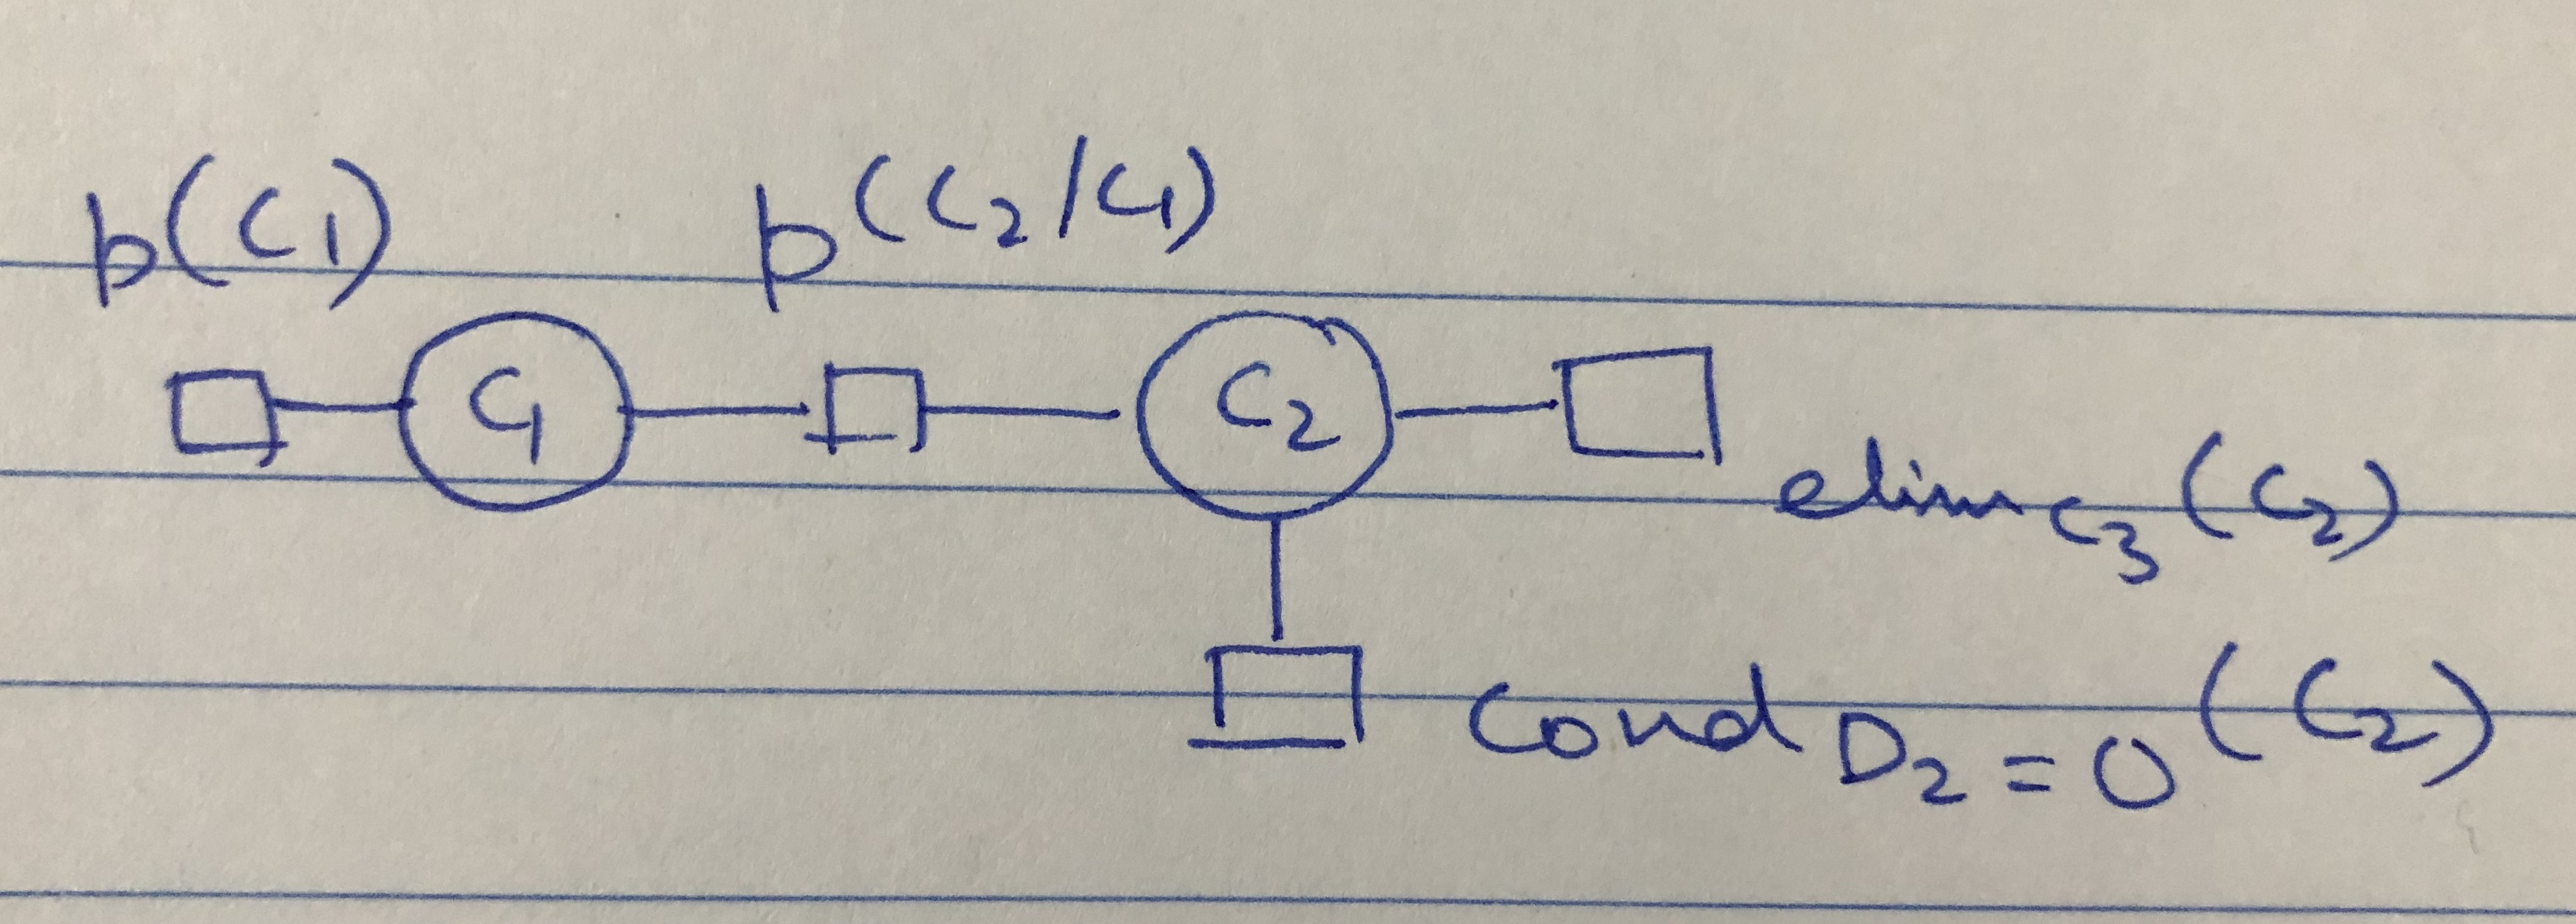
\includegraphics[scale=0.1]{IMG_2282.jpg}
  \end{center}
  Condition variable $D_2$ on value $D_2 = 0$, replacing it with a factor cond$_{D_2 = 0}(C_2)$, we get
  \begin{center}
  \begin{tabular}{ll}
  cond$_{D_2 = 0}(C_2)$ & $C_2$  \\
  $1-\eta$            & 0       \\
  $\eta$               & 1       \\
  \end{tabular} \newline \\
  \end{center}
  
  
  \textbf{Step6: Eliminate $C_1$} \\
  \begin{center}
  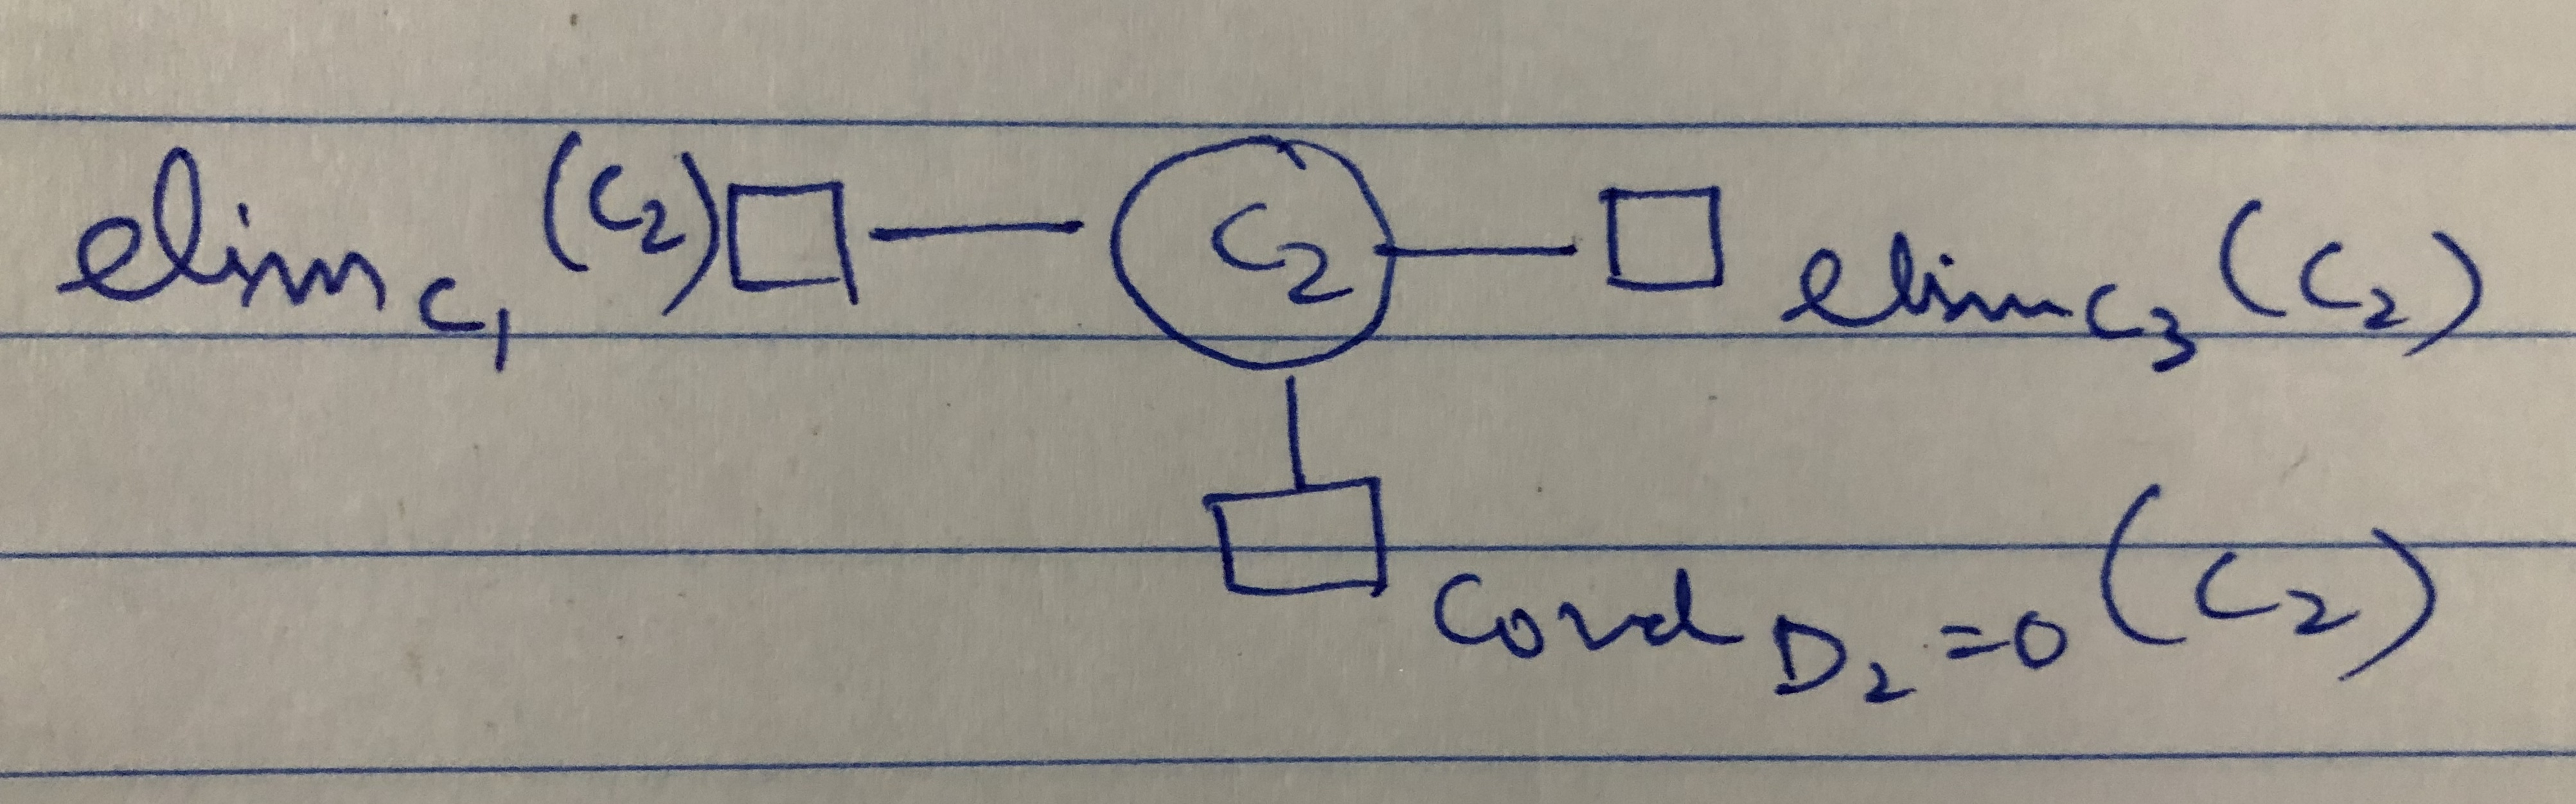
\includegraphics[scale=0.1]{IMG_2283.jpg}
  \end{center}
  \begin{align*}
	elim_{C_1}(C_2) &= \sum_{C_1} p(C_1) p(C_2/C_1) \\
	&= 0.5 \sum_{C_1} p(C_2/C_1)
  \end{align*}
  This is given from the below table:
  \begin{center}
  \begin{tabular}{ll}
  elim$_{C_1}(C_2)$ & $C_2$  \\
  $0.5(1-\epsilon + \epsilon) = 0.5$            & 0       \\
  $0.5(\epsilon + 1-\epsilon) = 0.5$               & 1       \\
  \end{tabular} \newline \\
  \end{center}
  
  \textbf{Step7: Combining all factors of $C_2$} \\
    Therefore, now that we know elim$_{C_1}(C_2)$, cond$_{D_2 = 0} (C_2)$ and elim$_{C_3}(C_1)$,
  \begin{align*}
  p(C_2/ D_2 = 0, D_3 = 1) &= \text{elim}_{C_1}(C_2) * \text{cond}_{D_2 = 0} (C_2) * \text{elim}_{C_3}(C_2)
  \end{align*}
  \begin{center}
  \begin{tabular}{ll}
  $p(C_2/ D_2 = 0, D_3 = 1)$ & $C_2$  \\
  $0.5((1 - \epsilon) \eta + \eta (1- \epsilon)) (1 - \eta)$            & 0       \\
  $0.5(\epsilon \eta + (1- \eta) (1 - \epsilon)) \eta$               & 1       \\
  \end{tabular} \newline \\
  \end{center}
  Therefore, 
  \begin{align*}
  P(C_2 = 1/D_2 = 0, D_3 = 1) &= \frac{0.5 (\epsilon \eta + (1- \eta) (1 - \epsilon)) \eta}{0.5(\epsilon \eta + (1- \eta) (1 - \epsilon)) \eta + 0.5 ((1 - \epsilon) \eta + \epsilon (1- \eta)) (1 - \eta)} \\
  &= \frac{(\epsilon \eta + (1- \eta) (1 - \epsilon)) \eta}{(\epsilon \eta + (1- \eta) (1 - \epsilon)) \eta + ((1 - \epsilon) \eta + \epsilon (1- \eta)) (1 - \eta)}
  \end{align*}
  \item
  \begin{enumerate}[label=\roman*.]
  \item
  \begin{align*}
  P(C_2 = 1/D_2 = 0) &= 0.2 \\
  P(C_2 = 1/D_2 = 0, D_3 = 1) &= 0.4157
  \end{align*}
  \item
  Adding second sensor reading increased the probability from $0.2$ to $0.4157$. Since $D_3$ is equal to 1, it means we observed the location to be 1 at location 3. This would increase the probability of $C_3 = 1$ since the emission probability $p(d_t/c_t)$ favours similar values with higher probability. $C_3 = 1$ increases the probability of $C_2 = 1$, since the transition probability $p(c_t/c_{t-1})$ favours same location with higher probability.
  \item Both the probabilities would be same when the sensor reading at $D_3$ doesn't matter. This won't matter when the transition probabilities $p(c_t/c_{t-1})$ are equal meaning no matter what is the value of $c_3$ out of all the possible values, we will get constant transition probability. This would happen when $\epsilon = 1 - \epsilon$, therefore when $\epsilon = 0.5$. 
  
  \end{enumerate}
\end{enumerate}

\section*{Problem 5}

\begin{enumerate}[label=(\alph*)]
  \item Simplifying the equation $P (C_{11}, C_{12} | E_1)$ using the Bayes Theorem, we have
  \begin{align*}
  P (C_{11}, C_{12} | E_1) &= P(C_{11}/E_1| C_{12}/E_1) * P(C_{12}/E_1)
  \end{align*}
  Since the location of both the cars are independent of each other ($C_{11}$ doesn't depend in any way on $C_{12}$ and vice versa), therefore, $C_{11}/E_1$ and $C_{12}/E_1$ are independent events.
  \begin{align*}
  P (C_{11}, C_{12} | E_1) &= P(C_{11}/E_1) * P(C_{12}/E_1)
  \end{align*}
  For the given question, we have to compute $P(C_{11}, C_{12} / E_1 = e_1)$. This means we are given a permutation $e_1$ out of possible domain values of $E_1$, which means observed distance of car 1 is $e_{11}$ and observed distance of car 2 is $e_{12}$.
    \begin{align*}
  P (C_{11}, C_{12} | E_1 = e_1) &= P(C_{11}/E_1 = e_1) * P(C_{12}/E_1 = e_1) \\
  &\propto p(c_{11})p_N (e_{11}, || a_1 - c_{11} ||, \sigma^2) * p(c_{12})p_N (e_{12}, || a_1 - c_{12} ||, \sigma^2)
  \end{align*}
  \item As per the solution in 5a, the joint probability would be defined as
  \begin{align*}
  &P (C_{11} = c_{11}, C_{12} = c_{12} ... C_{1K} = c_{1k} | E_1 = e_1) \\ &\propto p(c_{11})p_N (e_{11}, || a_1 - c_{11} ||, \sigma^2) * p(c_{12})p_N (e_{12}, || a_1 - c_{12} ||, \sigma^2) ... p(c_{1K}) p_N (e_{1K}, || a_1 - c_{1K} ||, \sigma^2) \\
& \propto p(c_{1i})^K \prod_{j=1}^{K} p_N(e_{1j}, || a_1 - c_{1j} ||, \sigma^2)
  \end{align*}
  Since $e_1$($(e_{11}, e_{12} ... e_{1k})$) is one set of readings from the list of all readings in $E_1$, therefore, in order to find the maximum value of the above equation, the minimum number of assignments to find maximum probability would be the total number of possible permutations of different distances observed, namely $(D_{11}, D_{12} ... D_{1k})$ which are in $E_1$. For each permutation, we can compute the value of the above product and find out the permutation for which the product is the maximum. Therefore, permutations of $(D_{11}, D_{12} ... D_{1k})$ is: $D_{11}$ can be assigned in $k$ ways, $D_{12}$ can be assigned in $k-1$ ways and so on. Therefore, 
  \begin{align*}
  \textbf{Minimum assignments} &= k * (k-1) * (k-2) ... (2) (1) \\
  &= k!
\end{align*}
\item Converting to factor graph, it would look like the following for the posterior distribution over all K car locations at all T time steps conditioned on all sensor readings:
  \begin{center}
  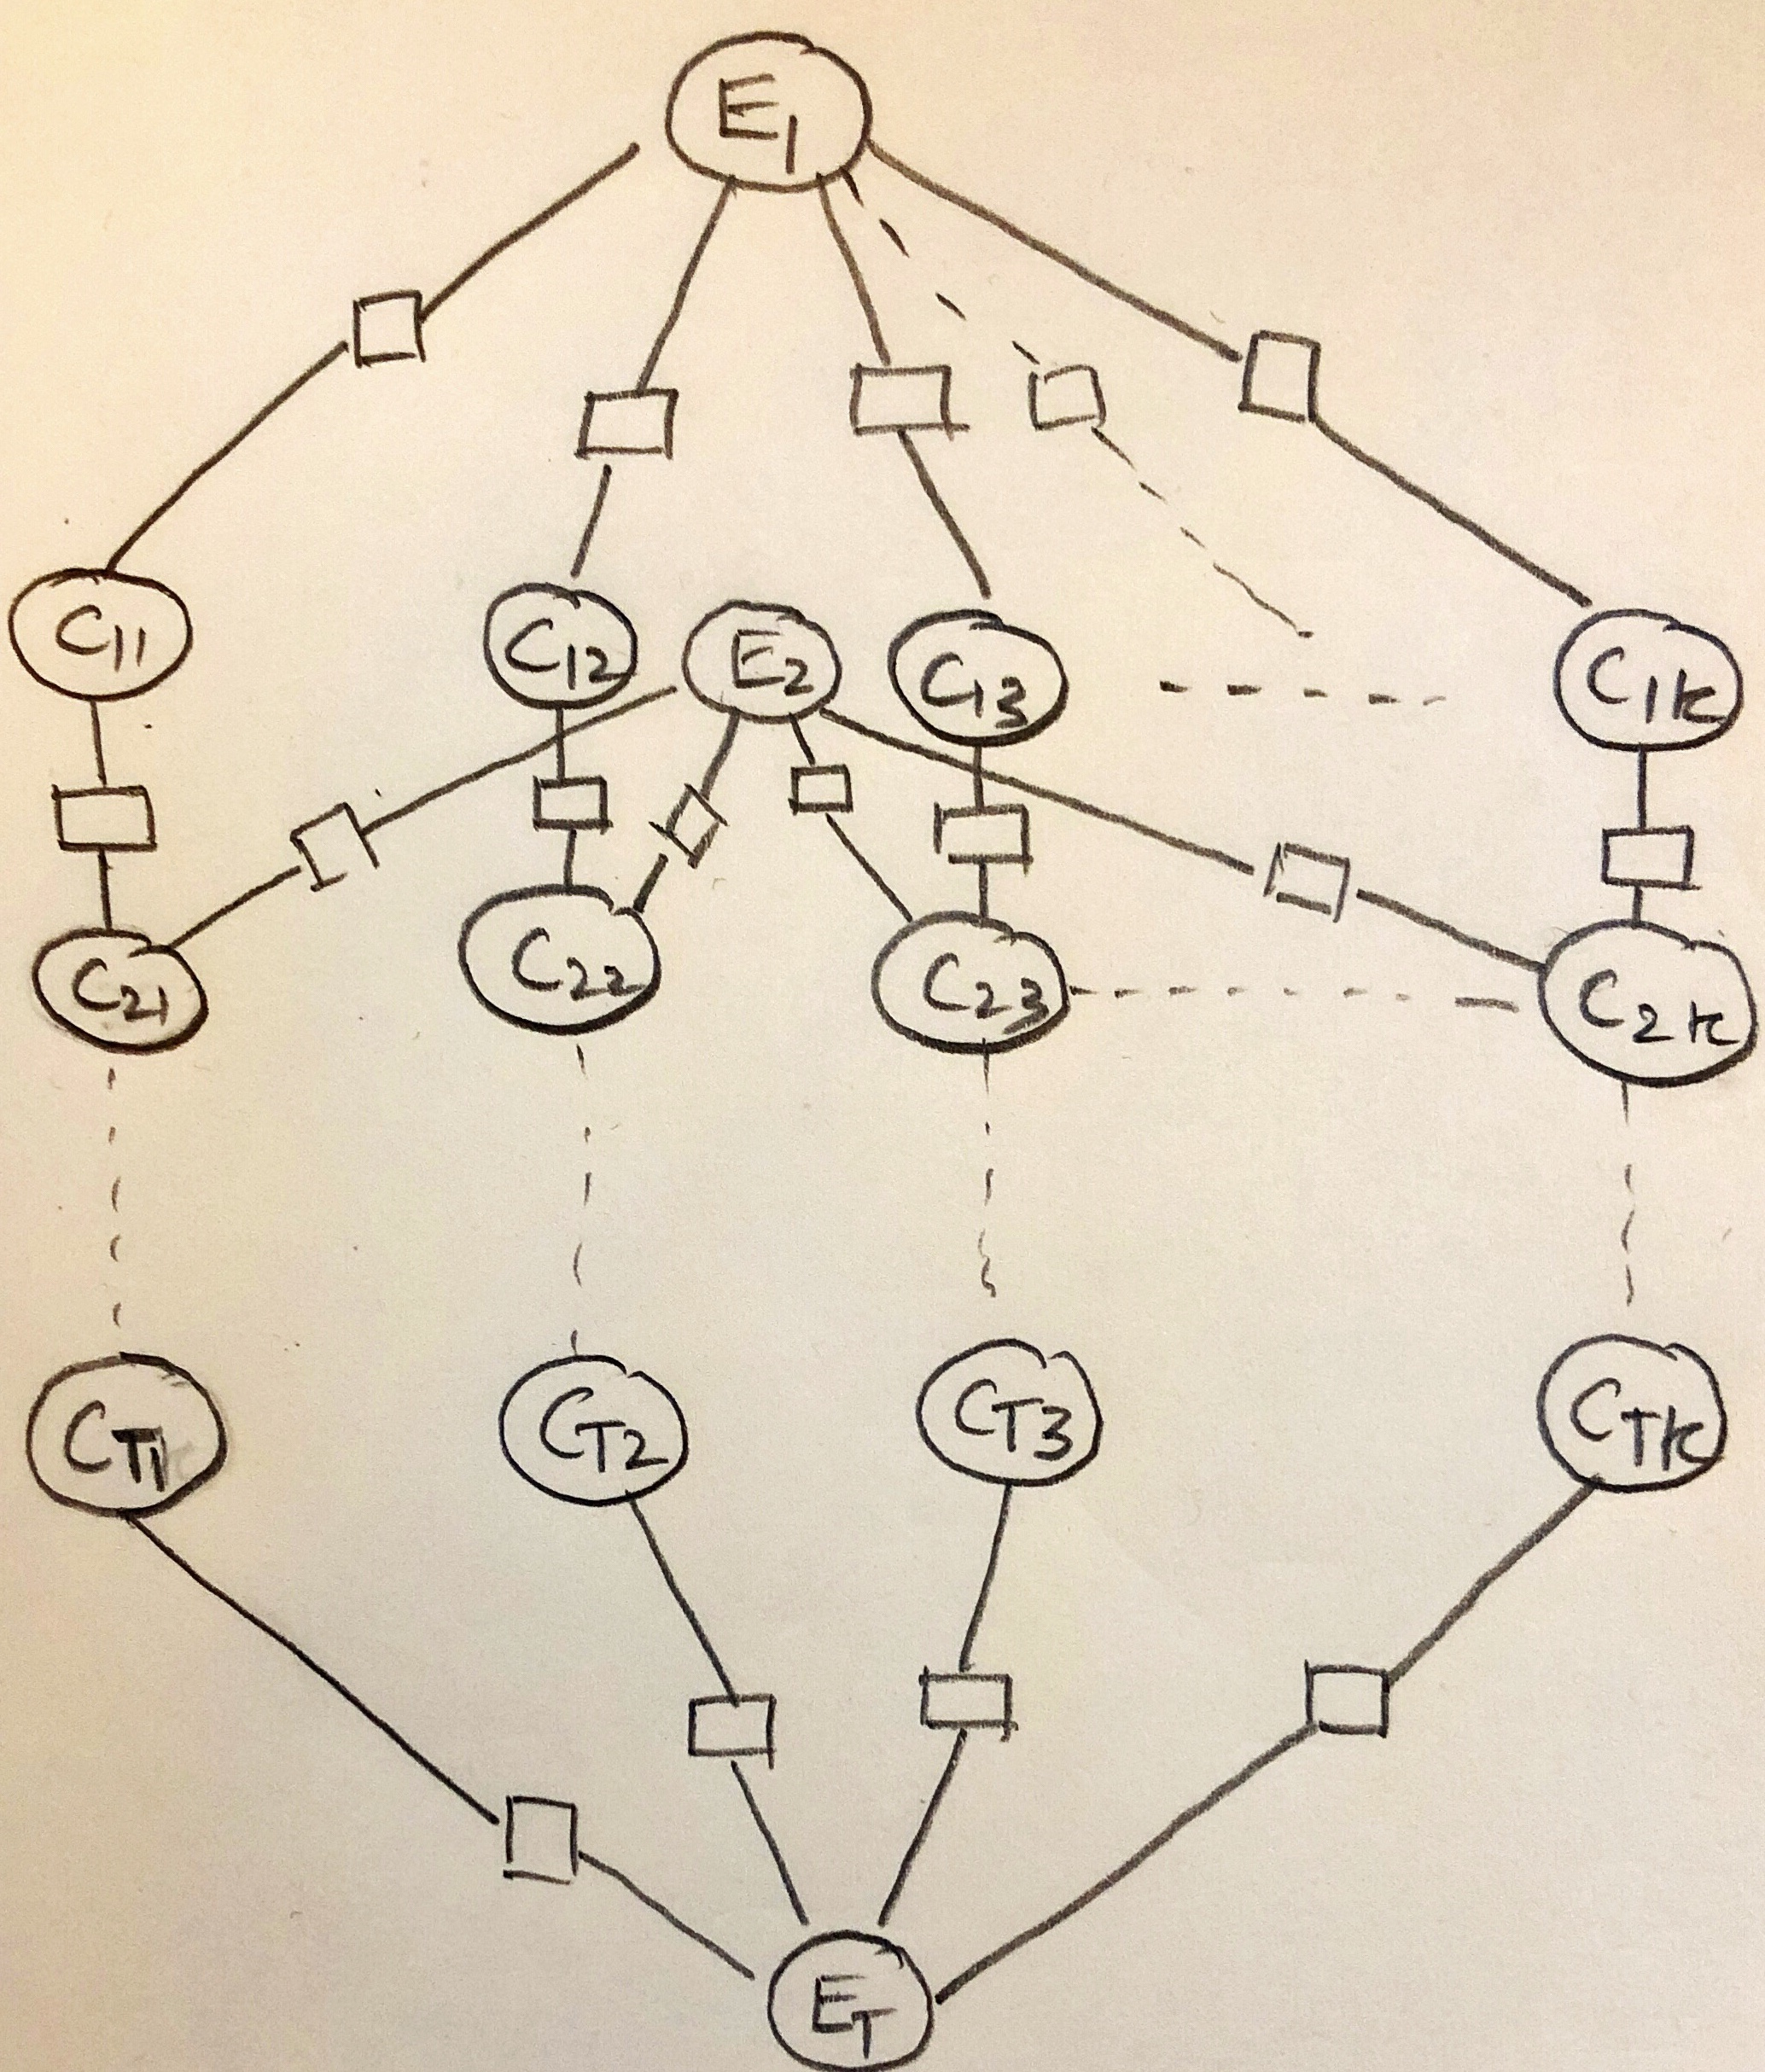
\includegraphics[scale=0.1]{IMG_2298}
  \end{center}
  
 \item In order to compute $p(c_{ti}/e_1, e_2, ... e_t)$, this would be a smoothening query in HMM. Domain of $C_{ti}$ would be the number of readings we get since those are exact values with equal probability of being assigned to $C_{ti}$, therefore has the domain $\{D_{t1}, D_{t2}, D_{t3} ... D_{tK}\}$. Following would be the lattice representation of this scenario:
   \begin{center}
  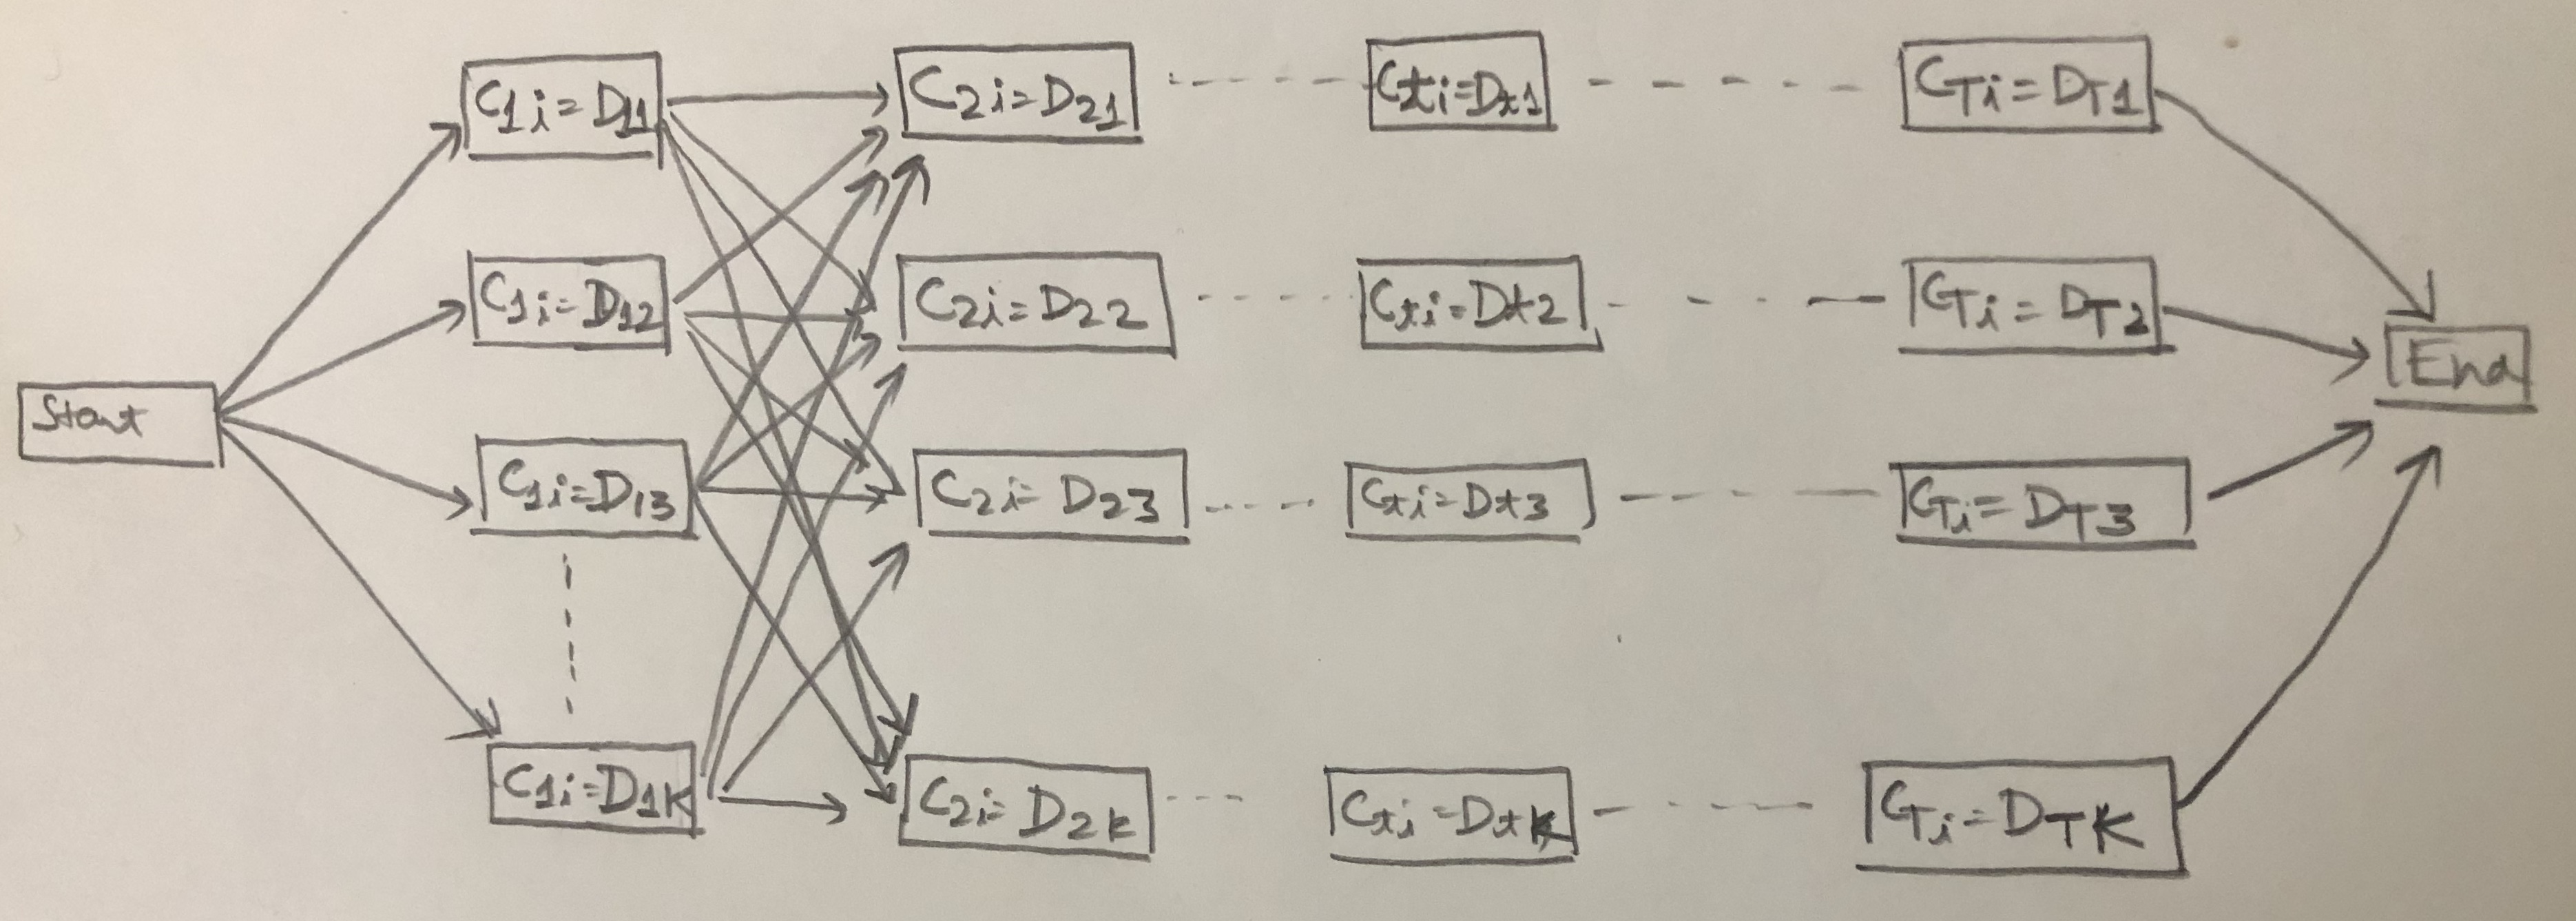
\includegraphics[scale=0.1]{IMG_2299}
  \end{center}
  We are interested in calculating the total number of paths which will pass through a particular value of $C_{ti}$, let's assume $D_{t1}$. This can be solved through Forward-Backward algorithm. \\ \\
  \textbf{Forward}
  \begin{align*}
  F_i(h_i) &= \sum_{c_{(t-1)i}} F_{i-1}(c_{(t-1)i}) w(c_{(t-1)i}, c_{ti})
  \end{align*}
  \textbf{Backward}
  \begin{align*}
  B_i(h_i) &= \sum_{c_{(t+1)i}} B_{i+1}(c_{(t+1)i}) w(c_{ti}, c_{(t+1)i})
  \end{align*}
  Finally we define $S_{i}(c_{ti}) = F_i(h_i) B_i(h_i)$, since it would be the sum of weights of paths from start to end. Finally we would normalise over the sum of the weights of all the possible paths from start to end.
  
  The algorithm would be as follows: \\
  Compute $F_1, F_2, F_3, ... F_t$ \\
  Compute $B_t, B_{t-1} ... B_{1}$ \\
  Compute $S_i$ for each $i$ and normalise.
 
\end{enumerate}

\end{document}